\documentclass[11pt,a4paper]{article}
\usepackage[utf8]{inputenc}
\usepackage{amsmath,enumitem,amsfonts,amssymb,graphicx,commath}
\usepackage{sectsty}
\usepackage{multicol}
\usepackage{tikz}
\usetikzlibrary{shapes,arrows,automata,arrows.meta}

\graphicspath{ {./img/} }
\DeclareMathAlphabet{\pazocal}{OMS}{zplm}{m}{n}

\usepackage[%
    left=1in,%
    right=1.0in,%
    top=0.8in,%
    bottom=1in,%
]{geometry}%

\sectionfont
{\fontsize{14.4}{12}\selectfont}
\title{\textbf{Principles of AI Planning
		\\{\Large Exercise Sheet 13}}}
\makeatletter
\renewcommand{\@maketitle}
{
	\newpage
	\null
	\vskip 2em%
	\begin{center}%
		{\LARGE \@title \\ \par}%
	\end{center}%
	\par
} \makeatother

\begin{document}
\begin{flushleft}
	Authors:\\
	Erick Rosete Beas | er165@uni-freiburg.de\\
	Jessica Lizeth Borja Diaz | jb986@uni-freiburg.de\\
\end{flushleft}
{\let\newpage\relax\maketitle}
\begin{center} 
	\large 07.02.2020
\end{center}


%%%%%%%%%%%%%%%%%%%%%  Ejercicio 1 %%%%%%%%%%%%%%%%%%%%%%%%%
\section*{Exercise 13.1 - EVMDDs}
(a)
\begin{multicols}{2}
	\begin{center}
		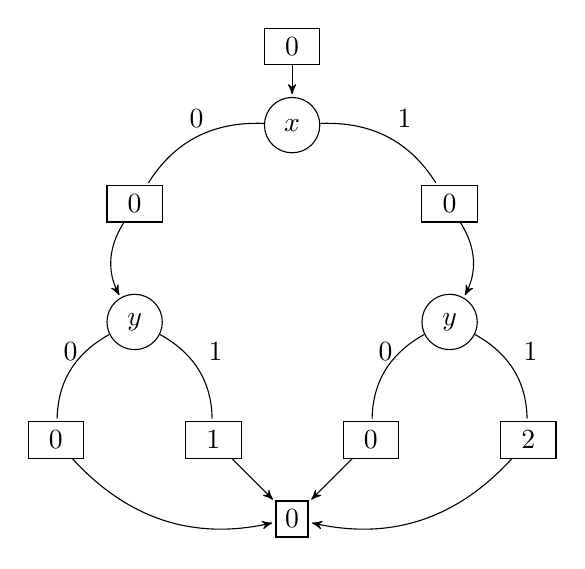
\begin{tikzpicture}
			\begin{scope}
				[
					styleVar/.style={
						minimum width = 2em, draw, circle,
						label={[above]#1}
						},
					styleCost/.style={minimum width = 2em, draw},
					end/.style={ minimum width = 0.2em, draw, thick},
				]
				\node(start)[styleCost] at (0,1) {$0$};
				\node(x)[styleVar] at (0,0) {$x$};
				\node(cx0)[styleCost] at (-2,-1) {$0$};
				\node(cx1)[styleCost] at (2,-1) {$0$};

				\node(y)[styleVar] at (-2,-2.5) {$y$};
				\node(cy0)[styleCost] at (-3,-4) {$0$};
				\node(cy1)[styleCost] at (-1,-4) {$1$};
				
				\node(yp)[styleVar] at (2,-2.5) {$y$};
				\node(cyp0)[styleCost] at (1,-4) {$0$};
				\node(cyp1)[styleCost] at (3,-4) {$2$};

				\node(end)[end] at (0,-5){$0$};
			\end{scope}
			\begin{scope}
				[ cost/.style = {->=stealth'},
				>=stealth',shorten >=1pt,auto]
				\path 
				(start) edge[cost]       		node{}(x)
				(x) edge[bend right, above]     node{$0$}(cx0)
				(x) edge[bend left]         	node{$1$}(cx1)
				(cx0) edge[bend right,cost]     node{}(y)
				(cx1) edge[bend left,cost]		node{}(yp)

				(y) edge[bend right, above]     node{$0$}(cy0)
				(y) edge[bend left]         	node{$1$}(cy1)
				(cy0) edge[bend right, cost]    node{}(end)
				(cy1) edge[cost]				node{}(end)

				(yp) edge[bend right, above]    node{$0$}(cyp0)
				(yp) edge[bend left]         	node{$1$}(cyp1)
				(cyp0) edge[cost]      		    node{}(end)
				(cyp1) edge[bend left, cost]    node{}(end);

			\end{scope}
		\end{tikzpicture}
	\end{center}
	\begin{center}
		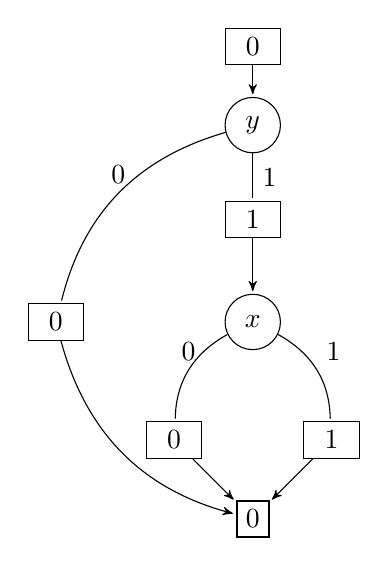
\begin{tikzpicture}
			\begin{scope}
				[
					styleVar/.style={
						minimum width = 2em, draw, circle,
						label={[above]#1},
						->=stealth'
						},
					styleCost/.style={minimum width = 2em, draw},
					end/.style={ minimum width = 0.2em, draw, thick},
				]
				\node(start)[styleCost] at (0,1) {$0$};
				\node(y)[styleVar] at (0,0) {$y$};
				\node(cy0)[styleCost] at (-2.5,-2.5) {$0$};
				\node(cy1)[styleCost] at (0,-1.2) {$1$};
	
				\node(x)[styleVar] at (0,-2.5) {$x$};
				\node(cx0)[styleCost] at (-1,-4) {$0$};
				\node(cx1)[styleCost] at (1,-4) {$1$};
				\node(end)[end] at (0,-5){$0$};
			\end{scope}
			
			\begin{scope}
				[ cost/.style = {->=stealth'},
					>=stealth',shorten >=1pt,auto]
				\path 
				(start) edge[cost] 					node{}(y)
				(y) edge[above, bend right]        	node{$0$}(cy0)
				(y) edge         					node{$1$}(cy1)
				(cy0) edge[bend right, cost]     	node{}(end)
				(cy1) edge[cost]			     	node{}(x)
	
				(x) edge[above,bend right]        	node{$0$}(cx0)
				(x) edge[bend left]         		node{$1$}(cx1)
				(cx0) edge[cost]				    node{}(end)
				(cx1) edge[cost]				    node{}(end);
	
			\end{scope}
		\end{tikzpicture}
	\end{center}
\end{multicols}
(b)
\begin{center}
	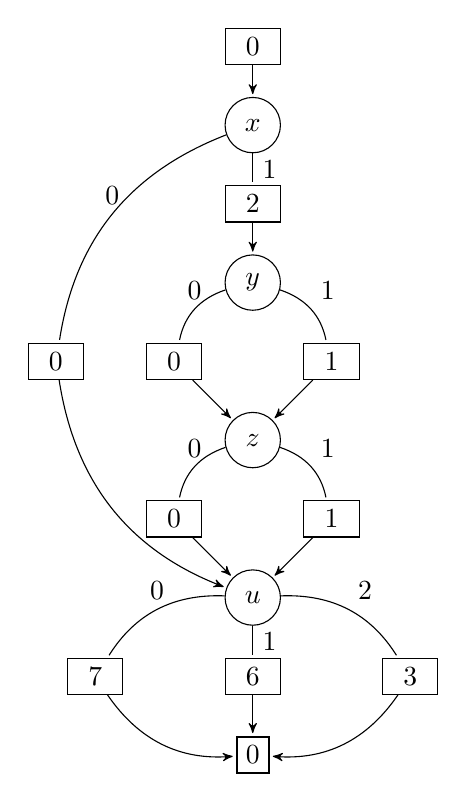
\begin{tikzpicture}
		\begin{scope}
			[
				styleVar/.style={
					minimum width = 2em, draw, circle,
					label={[above]#1},
					->=stealth'
					},
				styleCost/.style={minimum width = 2em, draw},
				end/.style={ minimum width = 0.2em, draw, thick},
			]
			\node(start)[styleCost] at (0,1) {$0$};
			\node(x)[styleVar] at (0,0) {$x$};
			\node(cx0)[styleCost] at (-2.5,-3) {$0$};
			\node(cx1)[styleCost] at (0,-1) {$2$};

			\node(y)[styleVar] at (0,-2) {$y$};
			\node(cy0)[styleCost] at (-1,-3) {$0$};
			\node(cy1)[styleCost] at (1,-3) {$1$};

			\node(z)[styleVar] at (0,-4) {$z$};
			\node(cz0)[styleCost] at (-1,-5) {$0$};
			\node(cz1)[styleCost] at (1,-5) {$1$};

			\node(u)[styleVar] at (0,-6) {$u$};
			\node(cu0)[styleCost] at (-2,-7) {$7$};
			\node(cu1)[styleCost] at (0,-7) {$6$};
			\node(cu2)[styleCost] at (2,-7) {$3$};

			\node(end)[end] at (0,-8){$0$};
		\end{scope}
		
		\begin{scope}
			[ cost/.style = {->=stealth'},
				>=stealth',shorten >=1pt,auto]
			\path 
			(start) edge[cost] 					node{}(x)
			(x) edge[bend right, above]        	node{$0$}(cx0)
			(x) edge         					node{$1$}(cx1)
			(cx0) edge[bend right, cost]     	node{}(u)
			(cx1) edge[cost]			     	node{}(y)

			(y) edge[bend right, above]        	node{$0$}(cy0)
			(y) edge[bend left]         		node{$1$}(cy1)
			(cy0) edge[cost]				    node{}(z)
			(cy1) edge[cost]				    node{}(z)

			(z) edge[bend right,above]        	node{$0$}(cz0)
			(z) edge[bend left]         		node{$1$}(cz1)
			(cz0) edge[cost]				    node{}(u)
			(cz1) edge[cost]				    node{}(u)

			(u) edge[bend right,above]        	node{$0$}(cu0)
			(u) edge			         		node{$1$}(cu1)
			(u) edge[bend left]         		node{$2$}(cu2)
			(cu0) edge[bend right, cost]		node{}(end)
			(cu1) edge[cost]				    node{}(end)
			(cu2) edge[bend left,cost]			node{}(end);

		\end{scope}
	\end{tikzpicture}
\end{center}
%%%%%%%%%%%%%%%%%%%%%  Ejercicio 2 %%%%%%%%%%%%%%%%%%%%%%%%%
\section*{Exercise 13.2 - EVMDD sizes and variable orders}


%%%%%%%%%%%%%%%%%%%%%  Ejercicio 3 %%%%%%%%%%%%%%%%%%%%%%%%%

%%%%%%%%%%%%%%%%%%%%%  Ejercicio 4 %%%%%%%%%%%%%%%%%%%%%%%%%

\end{document}